% !TEX root = ./HY-CS-main.tex
\chapter{Oppimisen analysoinnin tarpeet\label{oppimisenanalysoinnintarpeet}}

Oppimisanalytiikka tutkii oppimista ja opettamista oppimisympäristöissä ja hyödyntää analytiikkaa tunnistaessaan poikkeamia tai tehdessään muita oppijaa tukevia havaintoja \citep{longPenetratingFogAnalytics2011}. Vakiintunut oppimisanalytiikan määritelmä on 1st International Conference on Learning Analyticsin määritelmä \citep{siemensLearningAnalyticsEmergence2013,clowLearningAnalyticsCycle2012}: oppimisanalytiikka on oppijoista kerättävän datan mittaamista, keräämistä, analysointia ja raportointia, jota hyödynnetään oppimisen ja sen ympäristön ymmärtämiseen ja optimoimiseen.

Oppimisanalytiikkaa voidaan kuvata syklinä, jossa on neljä osa-aluetta: oppija, data, analyysi ja toiminta \citep{clowLearningAnalyticsCycle2012}. On tilanteita, joissa syklistä jää toiminta pois. Tälläisiä tilanteita ovat esimerkiksi raporttien muodostaminen oppimisdatasta, joiden pohjalta ei tehdä toimenpiteitä.

\begin{figure}[h]
    \centering
    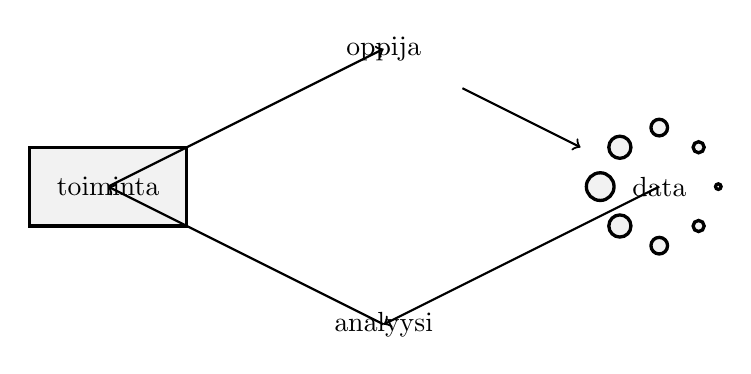
\begin{tikzpicture}
        \filldraw[color=black, fill=black!5, very thick] (-4.5,-0.5) rectangle (-2.5,0.5);

        \filldraw[color=black, fill=black!5, very thick] (4,0.5) circle (2pt);
        \filldraw[color=black, fill=black!5, very thick] (3.5,0.75) circle (3pt);
        \filldraw[color=black, fill=black!5, very thick] (3,0.5) circle (4pt);

        \filldraw[color=black, fill=black!5, very thick] (4,-0.5) circle (2pt);
        \filldraw[color=black, fill=black!5, very thick] (3.5,-0.75) circle (3pt);
        \filldraw[color=black, fill=black!5, very thick] (3,-0.5) circle (4pt);

        \filldraw[color=black, fill=black!5, very thick] (2.75,0) circle (5pt);
        \filldraw[color=black, fill=black!5, very thick] (4.25,0) circle (1pt);

        \node[] at (0,1.75) {oppija};
        \node[] at (3.5,0) {data};
        \node[] at (0,-1.75) {analyysi};
        \node[] at (-3.5,0) {toiminta};


        \draw[thick, ->] (1,1.25) -- (2.5,0.5);
        \draw[thick, ->] (3.5,0) -- (0,-1.75);
        \draw[thick, ->] (0,-1.75) -- (-3.5,0);
        \draw[thick, ->] (-3.5,0) -- (0,1.75);
    \end{tikzpicture}
    \caption{Oppimisanalytiikan eri vaiheet tiivistetysti \citep{clowLearningAnalyticsCycle2012}.}
\end{figure}

Syklissä oppija on oppimisanalytiikan lähtökohta \citep{clowLearningAnalyticsCycle2012}. Oppijoista kerätään dataa analytiikkaa varten, jota koostetaan erilaisista lähteistä \citep{wolffImprovingRetentionPredicting2013}. Oppimisympäristöstä saatavaa dataa voi olla esimerkiksi lokeihin kerätty tieto oppijan oppimisympäristössä liikkumisesta tai opintotietojärjestelmässä aiemmat kurssisuoritukset. Toisaalta myös oppijan oppimiskäyttäytymisen ja -tyylin ymmärtäminen ovat oppimisanalytiikassa keskistä \citep{hasanPredictingStudentPerformance2020}.

Oppijasta muodostunutta dataa voidaan tarkastella ja analysoida oppimisprosessin havainnollistamiseksi \citep{clowLearningAnalyticsCycle2012}. Tämä on oppimisanalytiikan tärkein vaihe. Oppijoista saatavan datan perusteella voidaan tunnistaa esimerkiksi putoamisvaarassa olevia opiskelijoita tai ennustaa heidän menestymistä kurssilla.

Oppimisanalytiikassa syklin viimeisen kohdan, toiminnan, on tarkoitus vaikuttaa oppijaan \citep{clowLearningAnalyticsCycle2012}. Toimintaa voi olla esimerkiksi oppijan käytössä oleva seurantanäkymä, jossa voi vertailla toisiin opiskelijoihin tai tarvittavan tuen kartoittaminen putoamisvaarassa olevalle opiskelijalle. Oppijan omien havaintojen ja opettajan havaintojen vaikutukset kohdistuvat oppijaan itseensä. Oppija voi hyödyntää analytiikasta saatavaa tietoa oman oppimisensa kehittämiseen hyvin nopeallakin vasteajalla.

Toiminta ei tavoita aina oppijaa, sillä tuloksia voidaan hyödyntää usealla tasolla \citep{clowLearningAnalyticsCycle2012}. Opettaja voi hyödyntää aiemman kurssi-iteraation kurssiarvosanoja kurssin kehittämisen tukena. Kurssin aikana opettajat toimet voivat vaikuttaa yhden oppijan sijasta myös useampaan oppijaan, ja opettajan toiminnan vaikutukset eivät välttämättä ole heti havaittavissa.

Hallintohenkilöstön toiminnan vaikutukset ovat laajempia ja hitaammin havaittavia heidän yhdistäessä myös opettajalta saatavan palautteen analyysiinsa \citep{clowLearningAnalyticsCycle2012}. Hallintohenkilöstö pystyy toiminnallaan vaikuttamaan isompaan joukkoon oppijoita kuin yksittäinen oppija esimerkiksi jakamalla kurssin kahteen osaan. Toisaalta oppimisanalytiikkaa voidaan hyödyntää laajemmalla tasolla esimerkiksi osana opetussuunnitelmatyötä, jolloin vaikutukset ovat vielä hitaammin havaittavissa, mutta niiden kattavuus on laajin \citep{clowOverviewLearningAnalytics2013}.

\color{blue}
Oppimisanalytiikaa voidaan hyödyntää kolmessa eri käyttötarkoituksessa, joita ovat kuvaileva analytiikka, ohjaava analytiikka ja ennustava analytiikka \citep{auvinenOppimisanalytiikkaTuleeOletko2017, danielBigDataAnalytics2015}. Kuvailevassa analytiikassa kuvaillaan ja analysoidaan oppijoista sekä muista oppimisen osa-alueista saatavaa historiatietoa. Kuvaileva analytiikka etsii esimerkiksi nykyisiä oppimistrendejä. Ennustava analytiikka puolestaan tarjoaa oppilaitoksille mahdollisuuden tehdä datan perusteella parempia päätöksiä ja näkymiä nykytilasta. Tavoitteena on estimoida tulevien tapahtumien todennäköisyyksiä. Ohjaava analytiikka puolestaan tarjoaa oppilaitoksille mahdollisuuden arvioida nykyistä toimintaansa vaihtoehtoisten mallien pohjalta ja ohjaa parempiin päätöksiin.
\color{black}

\color{red} Avaa tarpeita vielä lisää. \color{black}
